% textidote: ignore begin
\section{User interface}\label{sec:user-interface}
% textidote: ignore end

When designing the user interface, the group used an iterative approach.
This means that every iteration of the design was tested and evaluated by the group members or by other groups.
The group members would then discuss the design and decide on changes to be made.

\subsection{Brainstorming}\label{subsec:brainstorming}

Before starting on the actual design, the group agreed to have one brainstorming session, where everyone would share
their ideas on how the user interface should look.
Each group member presented their ideas either verbally or through sketches.
From those ideas, the group agreed on a number of key features that the user interface should have.
Everyone agreed that the final interface should be in the form of a dashboard, and that the data from
the~\acrshort{epos} should be visualized in a form of a chart.

% textidote: ignore begin
\begin{figure}[H]
    \centering
    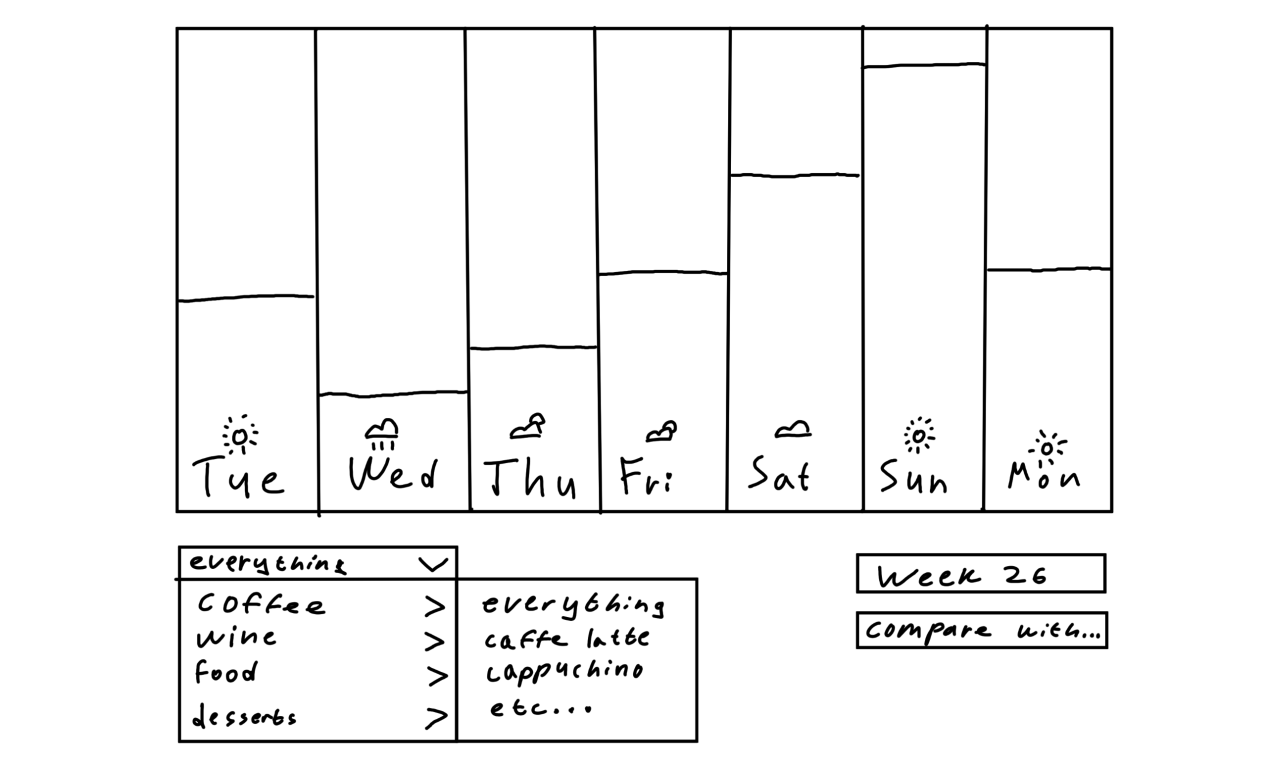
\includegraphics[width=\textwidth]{design-early.png}
    \caption{Navigation map of the final design.}\label{fig:design-early}
\end{figure}
% textidote: ignore end

The team decided on prioritizing two charts: A bar chart and a heatmap.
The functionality and choice rationale for these charts are explained in
Section~\ref{subsubsec:relevant-visualization-types}.
Figure~\ref{fig:design-early} shows an early prototype of a bar chart.
The designs and ideas were shared with the client, who approved of the direction the group was taking.

\subsection{Navigation map}\label{subsec:navigation-map}

After the brainstorming session, the group started to create a navigation map.
This map was made to visualize the flow of the user interface.
It features the different pages and how they are connected.
The navigation map can be seen in Figure~\ref{fig:navigation-map}.
Do note that the navigation map is representative of the final design and not the design of the prototypes.

The first page that the user interacts with is the login page.
From there they are taken to the dashboard, but they also have the choice to switch between the settings page and a list
of all the uploaded data.
The main focus for this project is the dashboard, where the user can see the different charts.
The settings page would allow the users to upload the data from their~\acrshort{epos} and to create categories for the
charts.
The total sales page shows a list of all the data without any visualization.
The user can also see visualization for a specific day from either the dashboard or the total sales page.

% textidote: ignore begin
\begin{figure}[H]
    \centering
    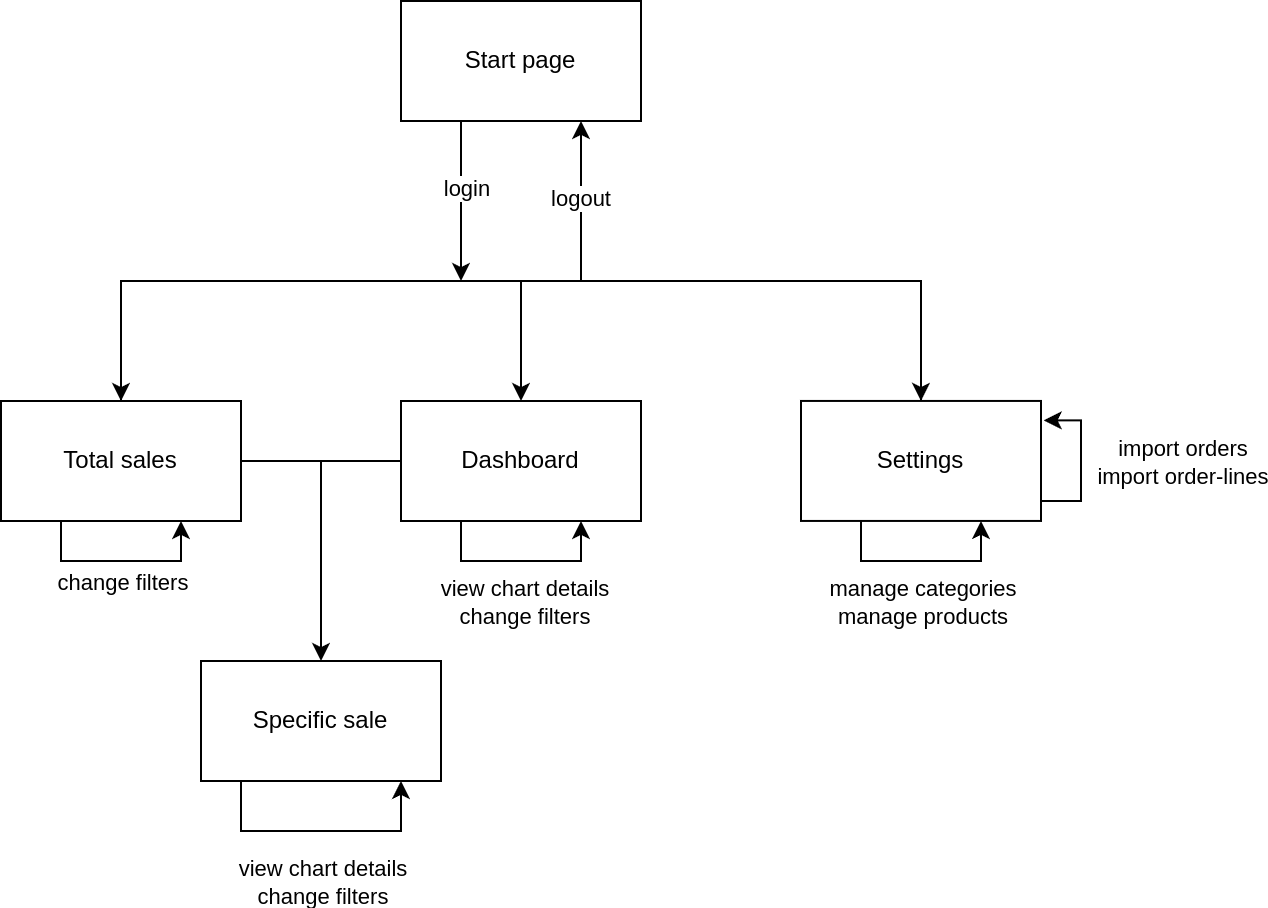
\includegraphics[width=\textwidth]{design-navigation-map.png}
    \caption{An example of an early chart.}\label{fig:navigation-map}
\end{figure}
% textidote: ignore end

\subsection{Lo-fi prototyping}\label{subsec:lo-fi-prototyping}

After the early prototyping phase, the group started to create a low-fidelity prototype.
This was done during a hackathon week, where the group had the opportunity to work on the prototypes together with
other groups.
Therefore, the group got a lot of feedback from other groups, which helped to improve the design.
The specific feedback is discussed in Section~\ref{sec:evaluation}.

This design, which can be seen in Figure~\ref{fig:lofi-prototype}, is made out of pen and paper.
It is made to be modular, which means that different charts and options can be attached or removed.
This encourages interactivity when testing the prototype.
The design focuses on a single chart at a time with an option to filter
the data using the calendar view on the bottom.
The charts can be switched between using the buttons on either side of the chart.
The calendar on the bottom can be clicked on to filter data for a specific time period.

% textidote: ignore begin
\begin{figure}[H]
    \centering
    \begin{subfigure}{.49\textwidth}
        \centering
        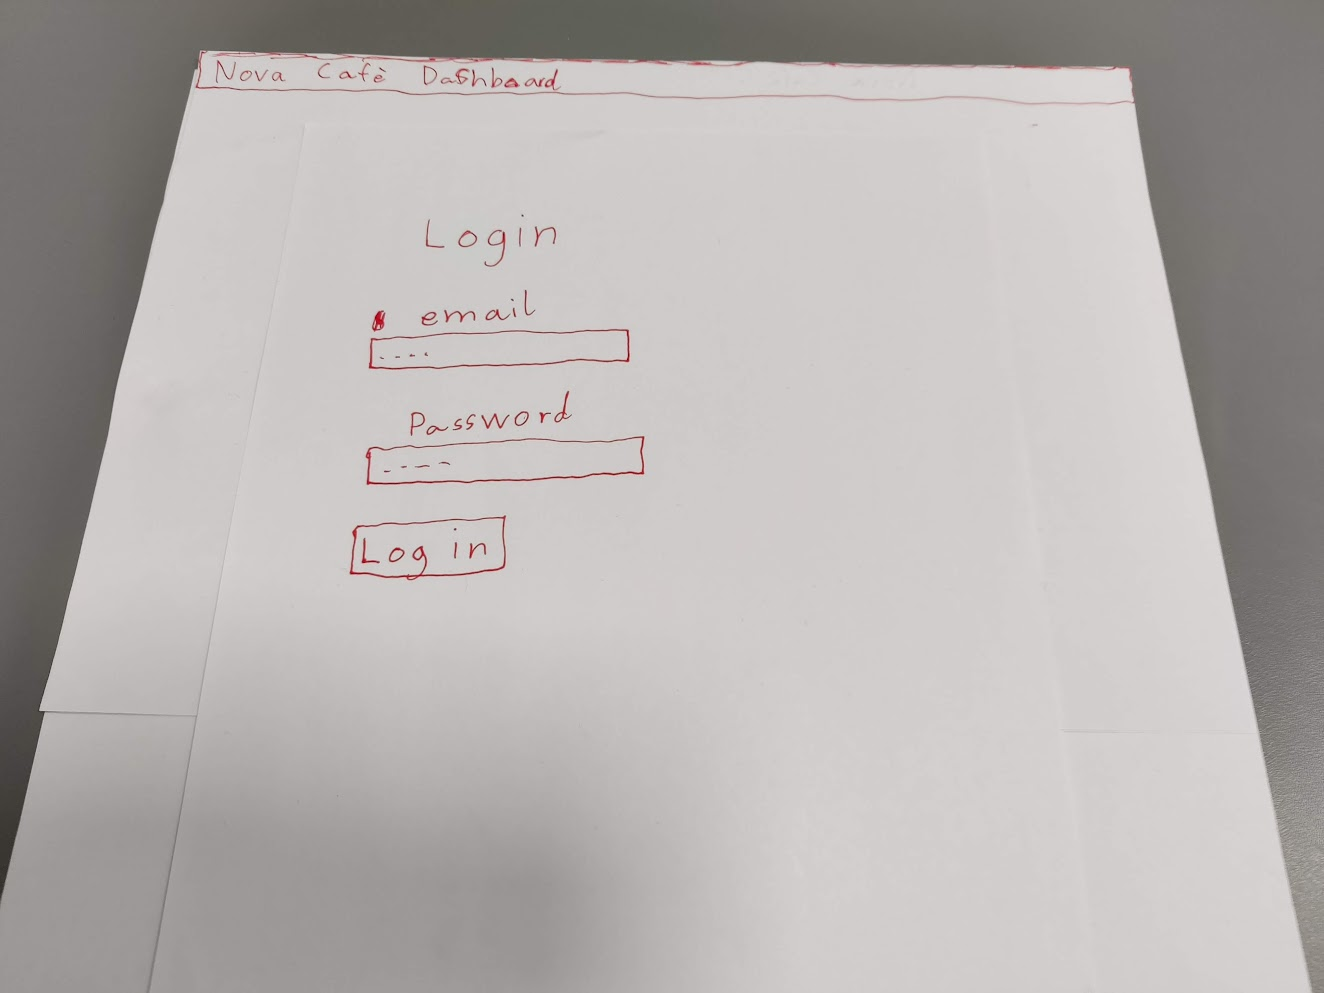
\includegraphics[width=\linewidth]{design-lofi-login.jpg}
        \caption{Login page.}\label{subfig:lofi-login}
    \end{subfigure}
    \begin{subfigure}{.49\textwidth}
        \centering
        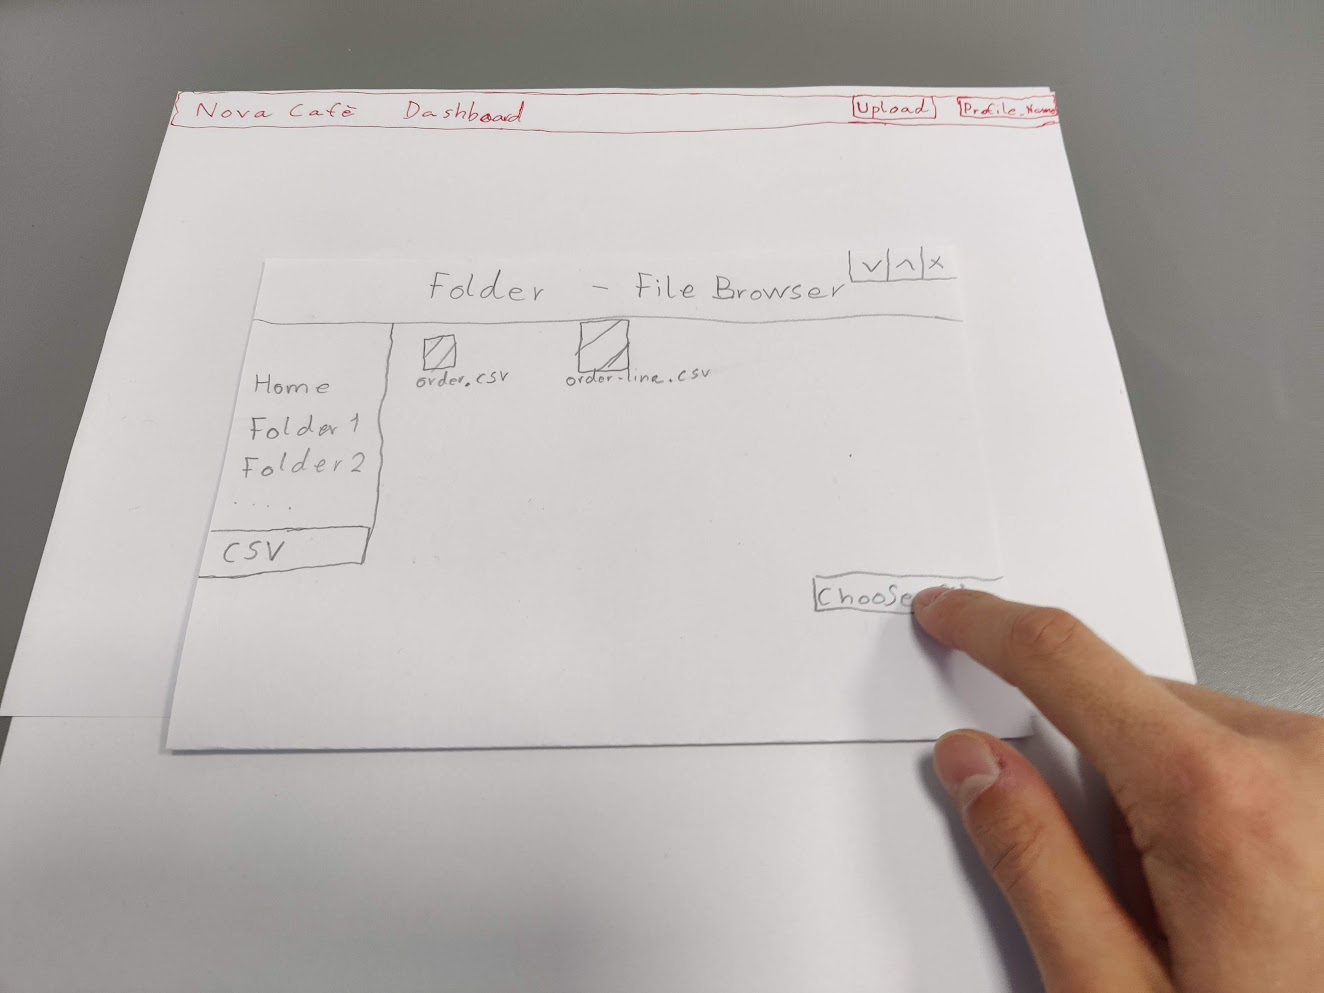
\includegraphics[width=\linewidth]{design-lofi-upload.jpg}
        \caption{Upload page.}\label{subfig:lofi-upload}
    \end{subfigure}
    \par\medskip
    \begin{subfigure}{.49\textwidth}
        \centering
        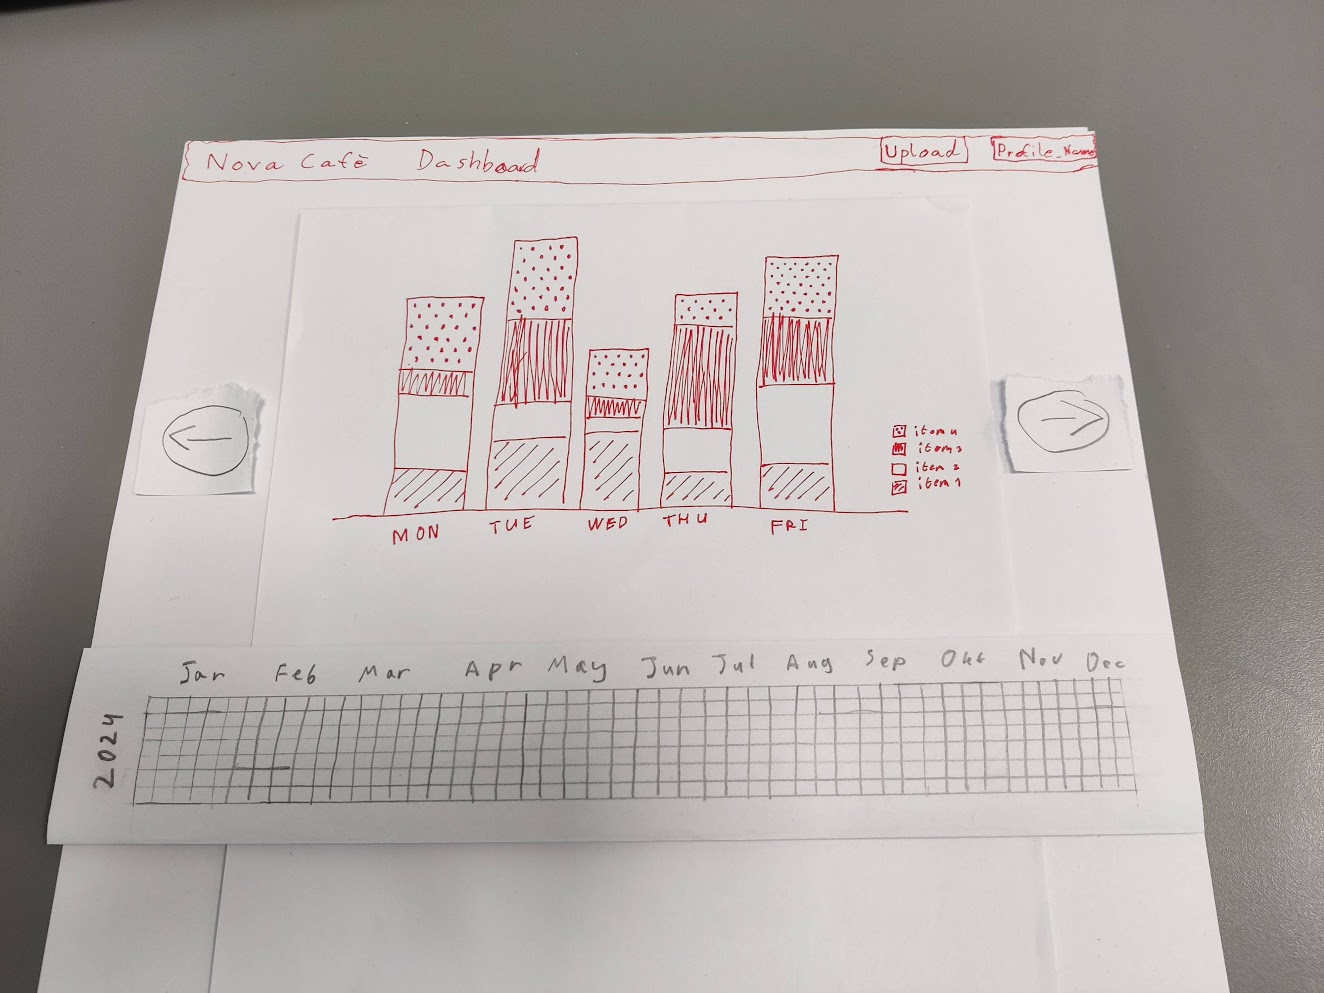
\includegraphics[width=\linewidth]{design-lofi-bar.jpg}
        \caption{Bar chart.}\label{subfig:lofi-bar}
    \end{subfigure}
    \begin{subfigure}{.49\textwidth}
        \centering
        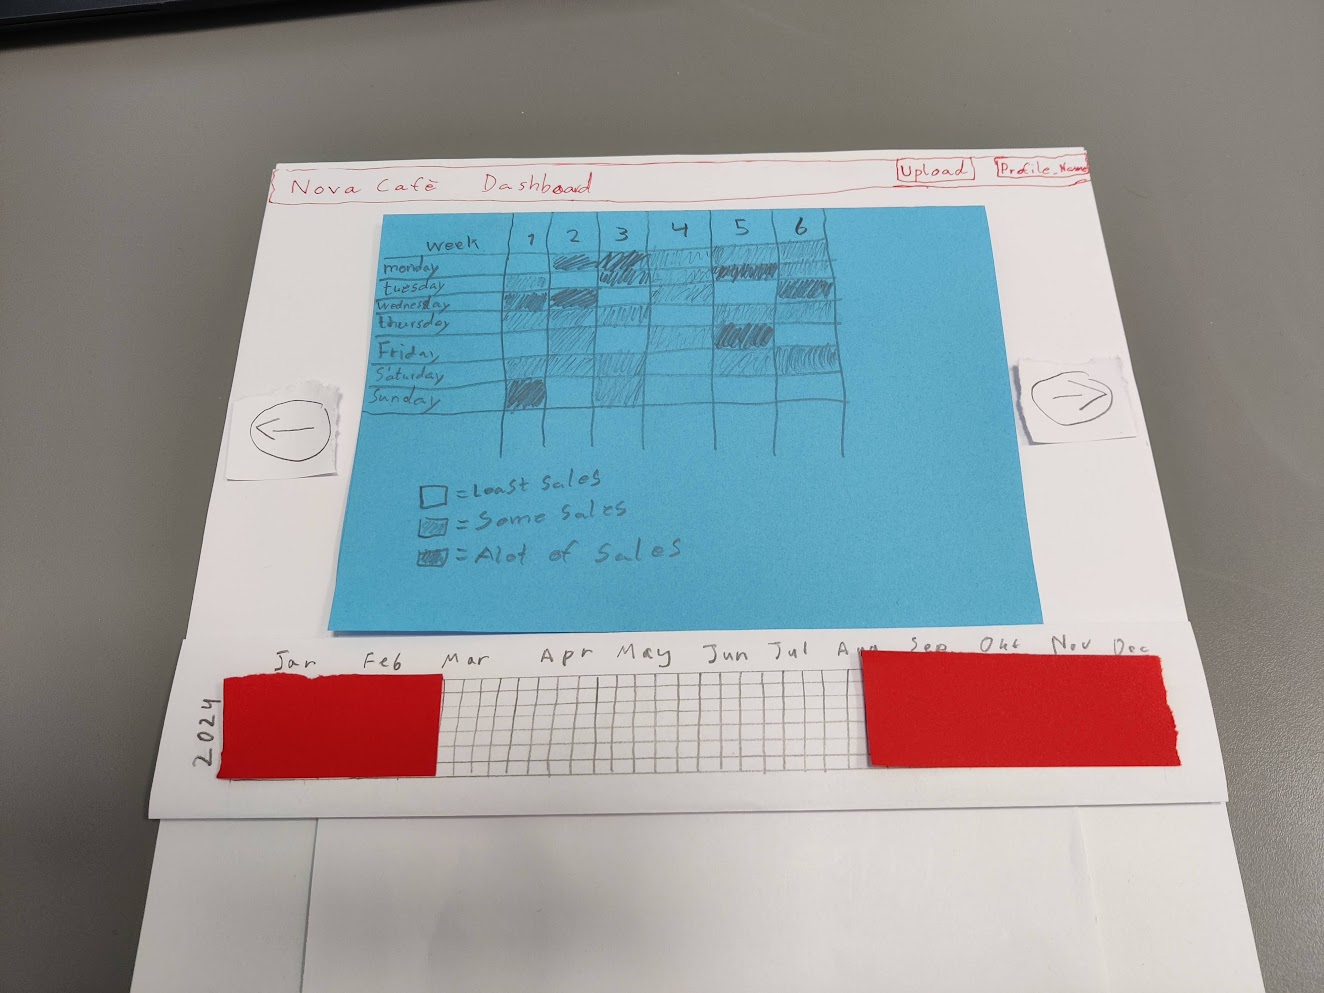
\includegraphics[width=\linewidth]{design-lofi-heatmap.jpg}
        \caption{Heatmap.}\label{subfig:lofi-heatmap}
    \end{subfigure}
    \caption{Lo-fi prototype}\label{fig:lofi-prototype}
\end{figure}
% textidote: ignore end

\subsection{Hi-fi prototyping}\label{subsec:hi-fi-prototyping}

During the course of the hackathon week, the group also made a high-fidelity prototype.
This prototype was made within the software solution itself, but without logic behind it and with mock data.
Doing this allowed for an easier transition from the prototype to the final product.
It also represented a more accurate experience of the final product, which made it easier to test and evaluate.

The hi-fi prototype, which can be seen in Figure~\ref{fig:hifi-prototype} is similar to the lo-fi prototype, but with a
more polished look.
The look of the charts is very close to the final design, minus a few minor changes that were made after the group
received feedback for the prototype.
This iteration does not communicate with the back-end, so the data is static.
It is also impossible to filter the data using the calendar view, as this feature would require a database connection.

The group could not implement the feedback they got for the lo-fi prototype, as the hi-fi prototype was made before
the feedback was received.
Instead, the feedback was used to improve the final design.

% textidote: ignore begin
\begin{figure}[H]
    \centering
    \begin{subfigure}{.75\textwidth}
        \centering
        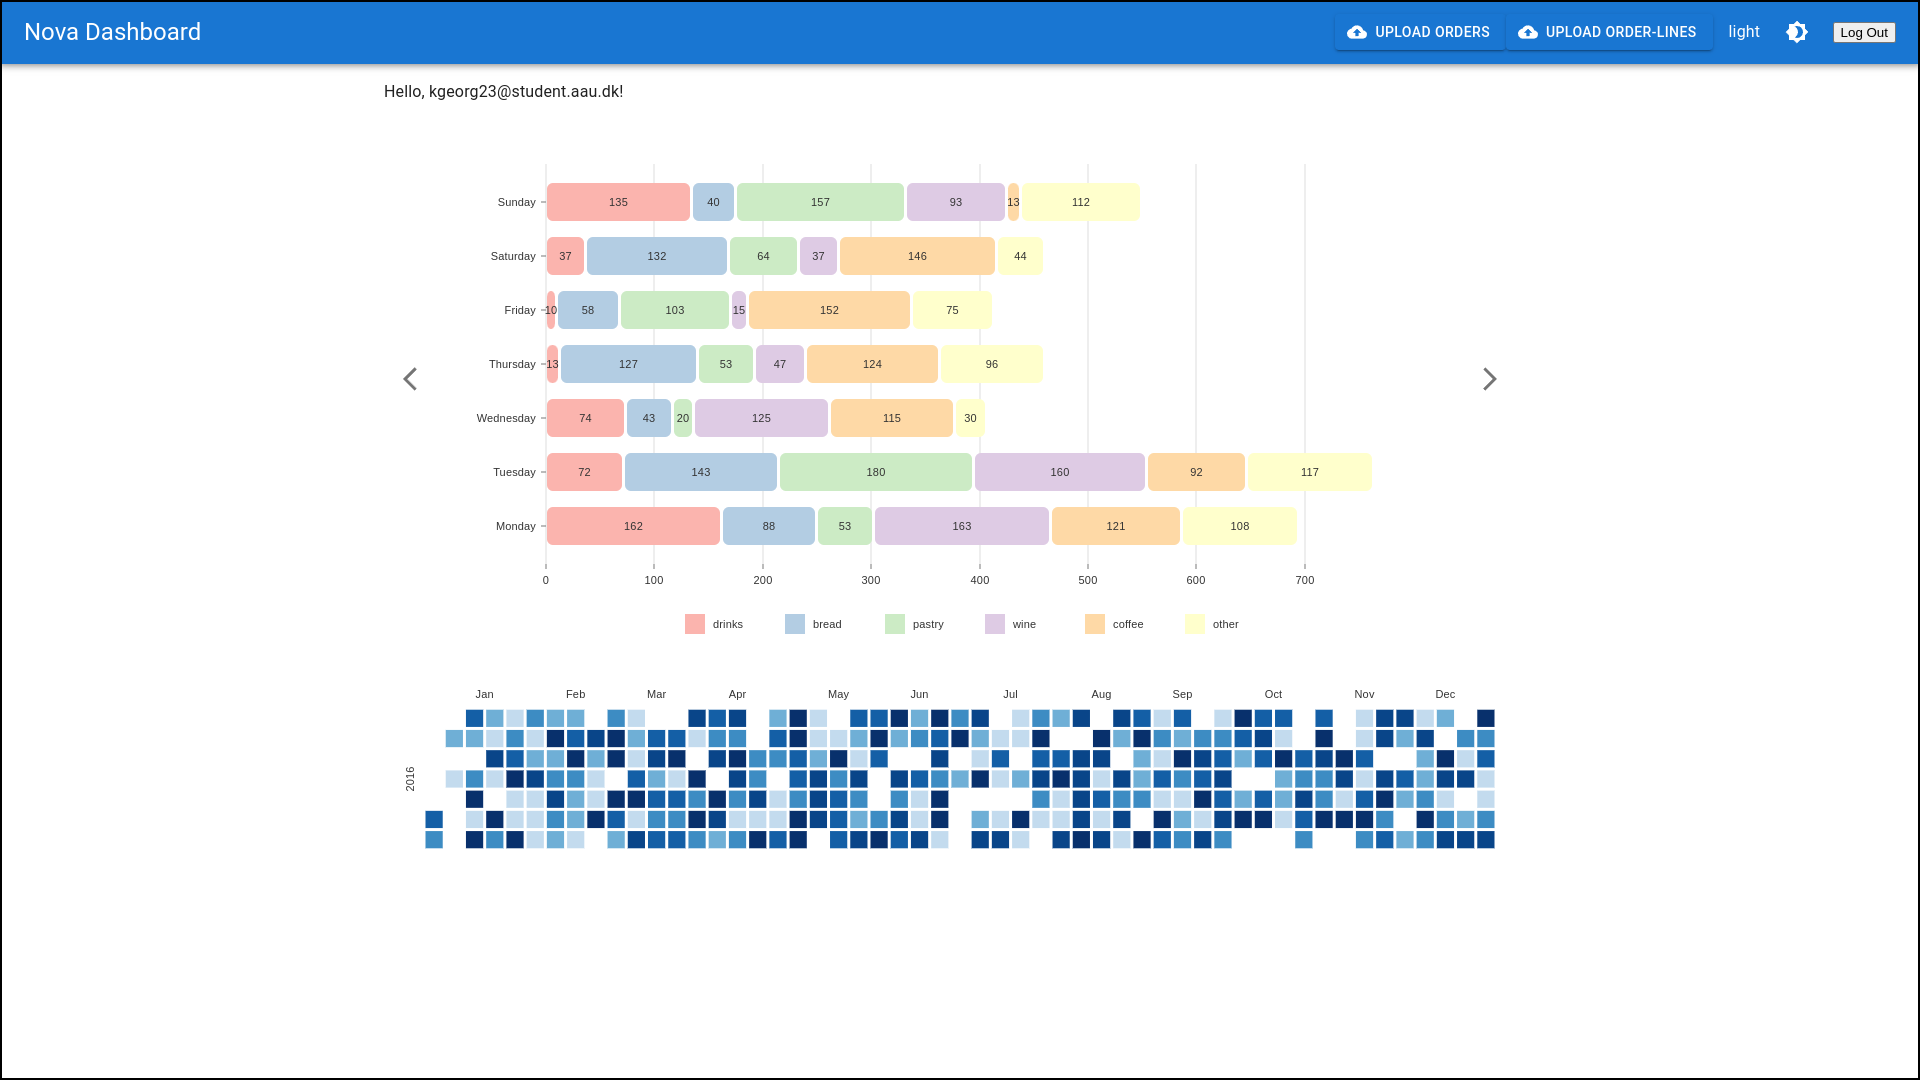
\includegraphics[width=\linewidth]{design-hifi-bar.png}
        \caption{Bar chart.}\label{subfig:hifi-bar}
    \end{subfigure}
    \par\medskip
    \begin{subfigure}{.75\textwidth}
        \centering
        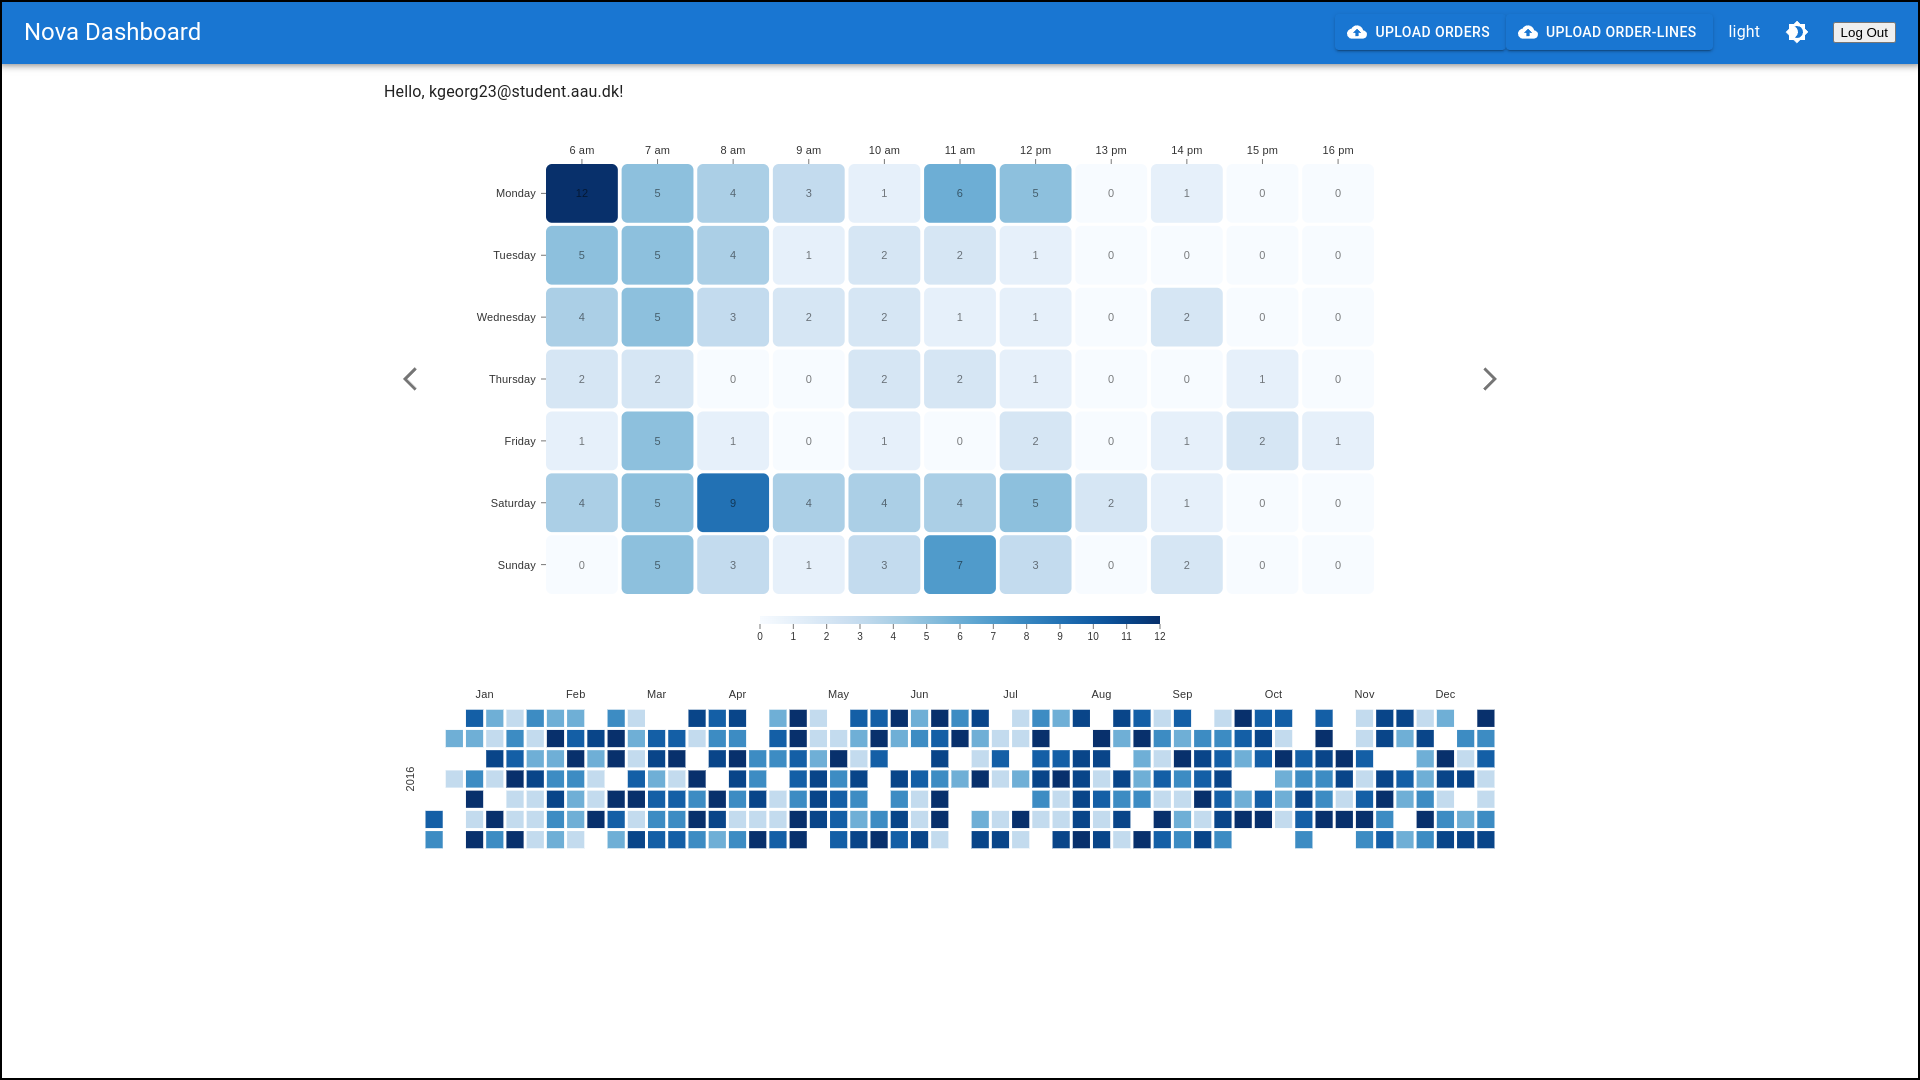
\includegraphics[width=\linewidth]{design-hifi-heatmap.png}
        \caption{Heatmap.}\label{subfig:hifi-heatmap}
    \end{subfigure}
    \caption{Hi-fi prototype}\label{fig:hifi-prototype}
\end{figure}
% textidote: ignore end

\subsection{Final design}

For the final design, the group went back to the hi-fi prototype and made some changes.
One request change was to show more charts on the dashboard at the same time.
This was done by making the charts smaller and adding charts below each other.
The filter options are now a button instead to allow for more precise date filtering.
Finally, the navigation bar was moved from the top to the side of the page to allow for more space for the charts.
The bar is also collapsible if the user wants to focus on the charts.

The group took into consideration their target audience when designing the user interface.
The interface is minimalistic, and the colors are simple to appeal to the co-workers at the café are mostly young adults.
For gradient transitions, the group is using shades of blue, with darker shades representing higher values and lighter
shades representing lower values.
Blue was chosen as it contrasts well with its shades, which makes it easy to read the charts.
For variable colors, the group is using different colors that are easy to distinguish from each other.
An example of this can be seen in the bar chart, where the color of each bar is contrasting with the adjacent bars.
This was done to make it easier to distinguish between the different bars and to make the charts more accessible to
colorblind users.

% TODO insert final images
